\documentclass[10pt]{beamer}
%\documentclass[handout,10pt]{beamer}
%\mode<presentation>
%{
%  \usetheme{Berkeley}
%  \usecolortheme{seahorse}
%  \usefonttheme{default}
%  \setbeamertemplate{navigation symbols}{}
%  \setbeamertemplate{caption}[numbered]
%}

\usetheme{metropolis}

\usepackage[english]{babel}
\usepackage[utf8x]{inputenc}
\usepackage{caption}
\usepackage{multirow}
\usepackage{mathrsfs}
\usepackage{graphicx}
\usepackage{amsmath}
\usepackage{graphicx}
\usepackage[compatibility=false]{caption}
\usepackage{subcaption}
\usepackage[normalem]{ulem}
\DeclareMathOperator{\tr}{tr}
\usepackage{textpos}
\usepackage{animate}

\title[FMSP Further Mathematics]{Conic Sections}
%\titlegraphic{\includegraphics[height=1.57cm]{logo.jpg}}
\author[Scott Morgan]{\textbf{Scott Morgan}}
\institute{\textit{Further Mathematics Support Programme - WJEC A-Level Further Mathematics} \\
\textit{13th January 2018}
\\ \\ \\
\textit{scott3142.com | @Scott3142}}
\date

\begin{document}

\begin{frame}
  \maketitle
\end{frame}

\begin{frame}{Conic Sections}
  \begin{itemize}[<+->]
    \item Parabola
    \item Hyperbola
    \item Ellipse (\textit{special case: circle})
  \end{itemize}
\end{frame}

\begin{frame}{Conic Sections}
  \begin{figure}
    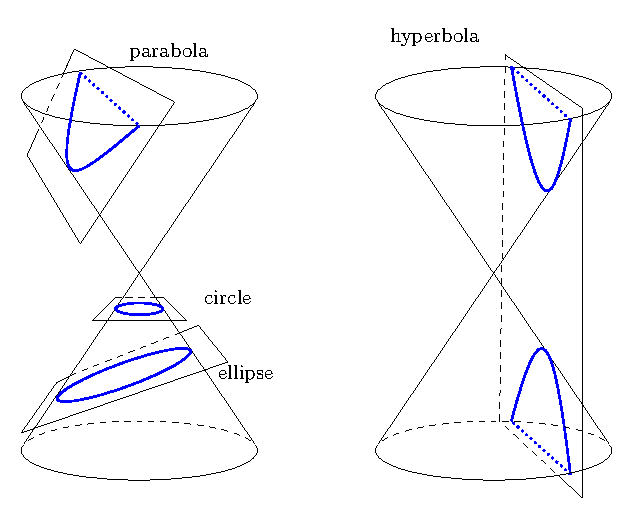
\includegraphics[scale=0.85]{examples/conics-example.pdf}
    \caption*{The reason they're called conic sections...}
  \end{figure}
\end{frame}

\begin{frame}{Key Words}
  \begin{itemize}[<+->]
    \item Eccentricity (usually denoted by $e$)
    \item Focus/Foci
    \item Directrix/Directrices
    \item Asymptotes
  \end{itemize}
\end{frame}

\begin{frame}{Directrix}
  \begin{figure}
    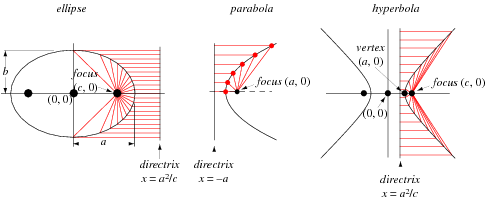
\includegraphics[width=\textwidth]{beamer-pics/directrix.png}
  \end{figure}
\end{frame}

\begin{frame}{Properties of Conic Sections - Parabola}

  \only<1>{
    \begin{figure}
      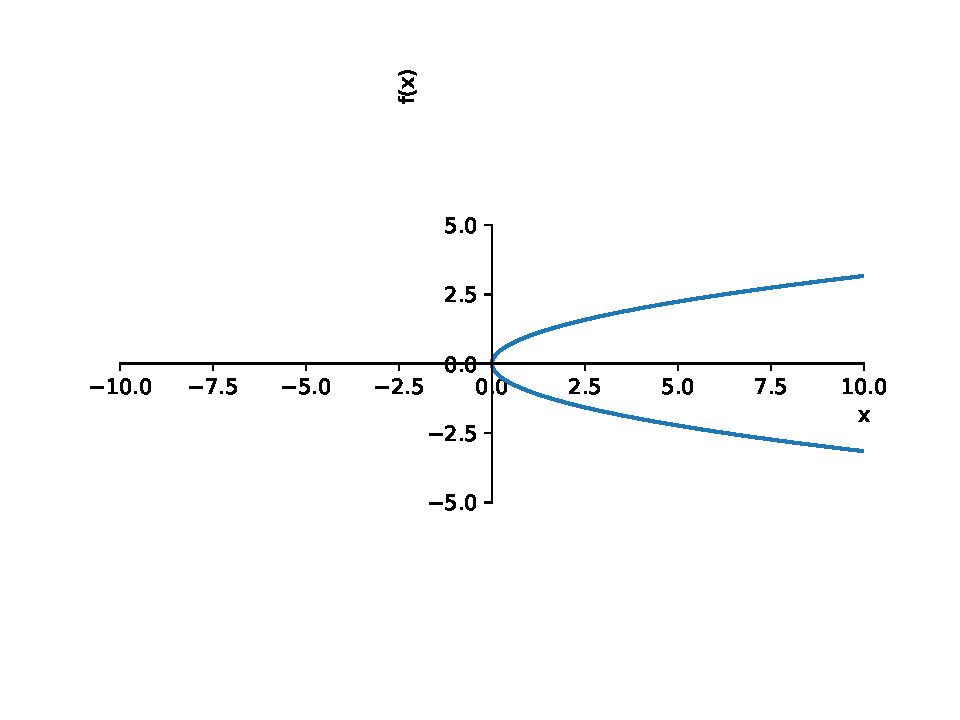
\includegraphics[width=\textwidth]{beamer-pics/conics-1.pdf}
    \end{figure}
  }

  \only<2->{
    \begin{columns}
      \begin{column}{0.5\textwidth}
        \begin{figure}
          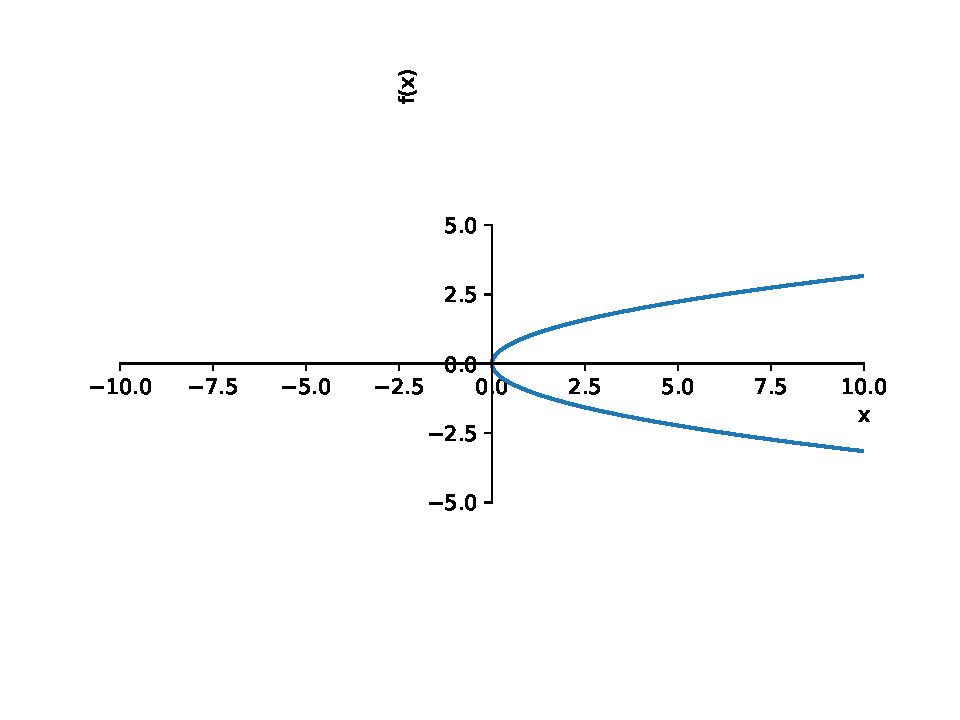
\includegraphics[width=\textwidth]{beamer-pics/conics-1.pdf}
        \end{figure}
      \end{column}

      \begin{column}{0.5\textwidth}
        \begin{itemize}[<+->]
          \item Equation (centre $(Q,R)$): $(y-R)^2 = 4a(x-Q)$
          \item Parametric form: $(Q+at^2,R+2at)$
          \item Eccentricity: $e = 1$
          \item Focus: $(a+Q,R)$
          \item Directrix: $x-Q = -a$
          \item Asymptotes: \textit{none}
        \end{itemize}
      \end{column}
    \end{columns}
  }
\end{frame}

\begin{frame}{Properties of Conic Sections - Hyperbola}
    \only<1>{
        \begin{columns}
          \begin{column}{0.5\textwidth}
            \begin{figure}
              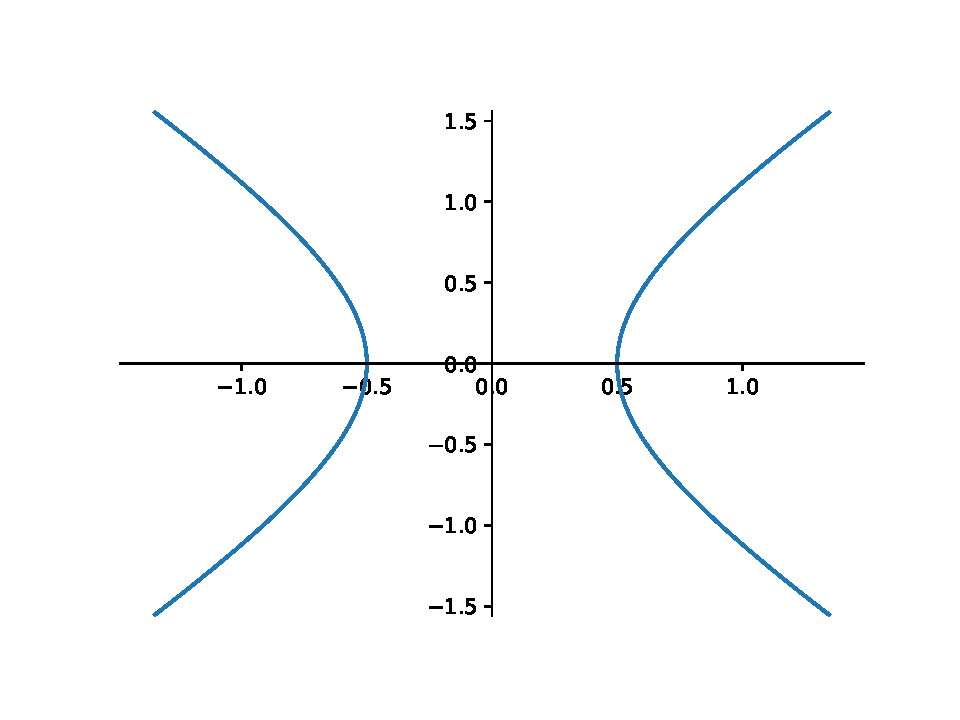
\includegraphics[width=\textwidth]{beamer-pics/conics-hyperbola-1.pdf}
            \end{figure}
          \end{column}

          \begin{column}{0.5\textwidth}
            \begin{figure}
              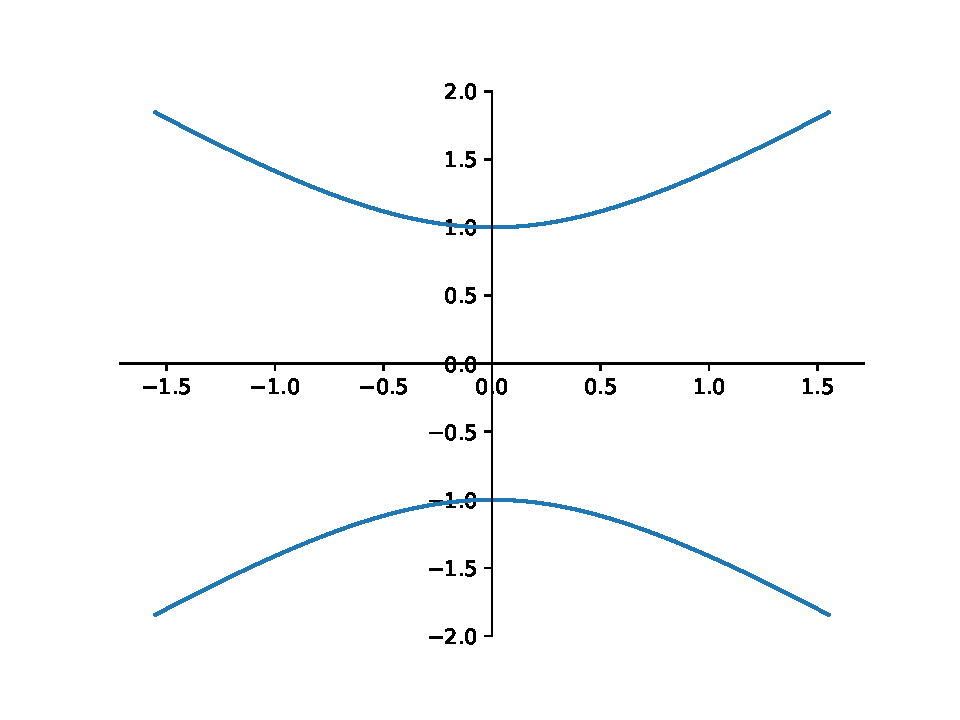
\includegraphics[width=\textwidth]{beamer-pics/conics-hyperbola-2.pdf}
            \end{figure}
          \end{column}
        \end{columns}
    }

    \only<2->{
      \begin{columns}
        \begin{column}{0.5\textwidth}
          \begin{figure}
            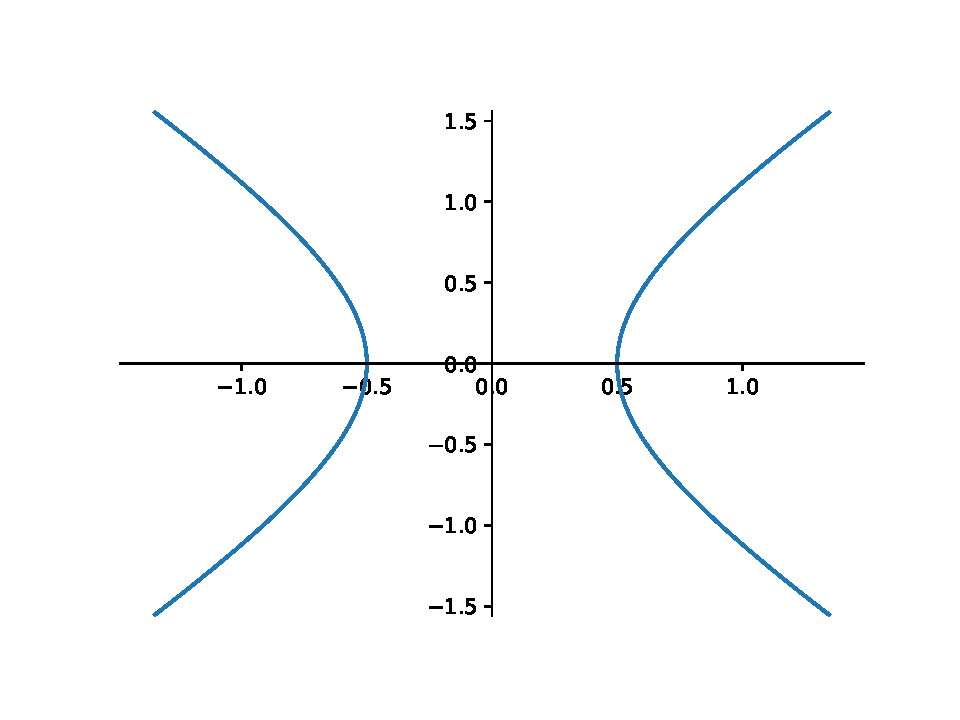
\includegraphics[width=\textwidth]{beamer-pics/conics-hyperbola-1.pdf}
          \end{figure}
        \end{column}

        \begin{column}{0.5\textwidth}
          \begin{itemize}[<+->]
            \item Equation (centre $(Q,R)$): $\frac{(x-Q)^2}{a^2} - \frac{(y-R)^2}{b^2} = 1$
            \item Parametric form: $(Q + a\sec\theta,R + b\tan\theta)$, $(Q + \pm a\cosh\theta,R + b\sinh\theta)$
            \item Eccentricity: $e > 1$, $b^2 = a^2(e^2-1)$
            \item Focus: $(Q \pm ae,R)$
            \item Directrices: $x-Q = \pm\frac{a}{e}$
            \item Asymptotes: $\frac{(x-Q)}{a} = \pm\frac{(y-R)}{b}$
          \end{itemize}
        \end{column}
      \end{columns}
    }
\end{frame}

\begin{frame}{Properties of Conic Sections - Ellipse}
   \only<1>{
        \begin{figure}
          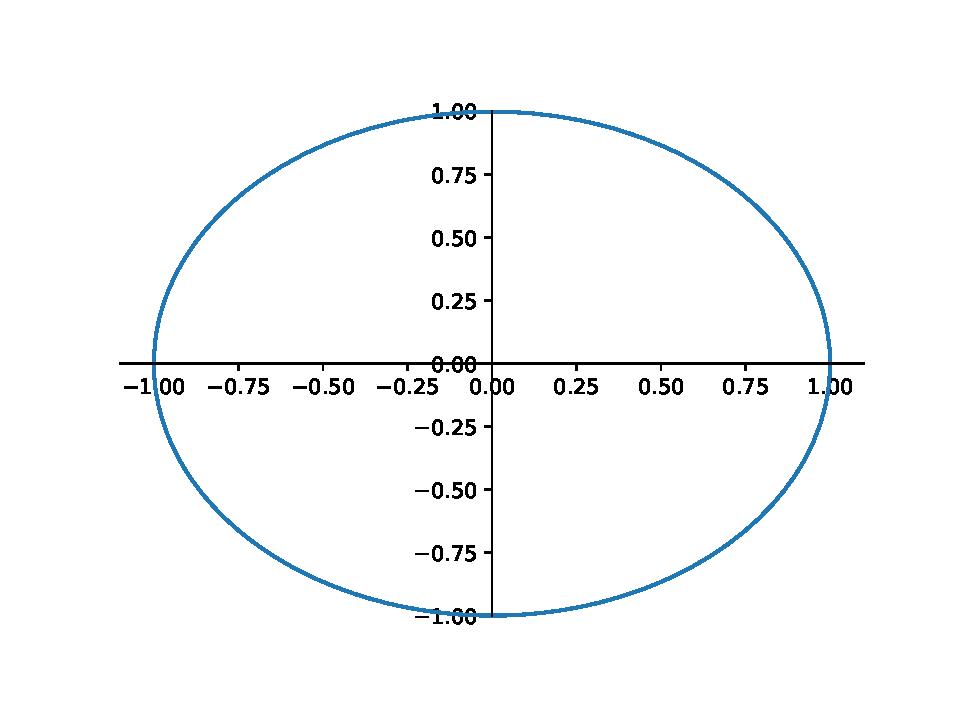
\includegraphics[width=0.9\textwidth]{beamer-pics/conics-ellipse.pdf}
        \end{figure}
    }

    \only<2->{
      \begin{columns}
        \begin{column}{0.5\textwidth}
          \begin{figure}
            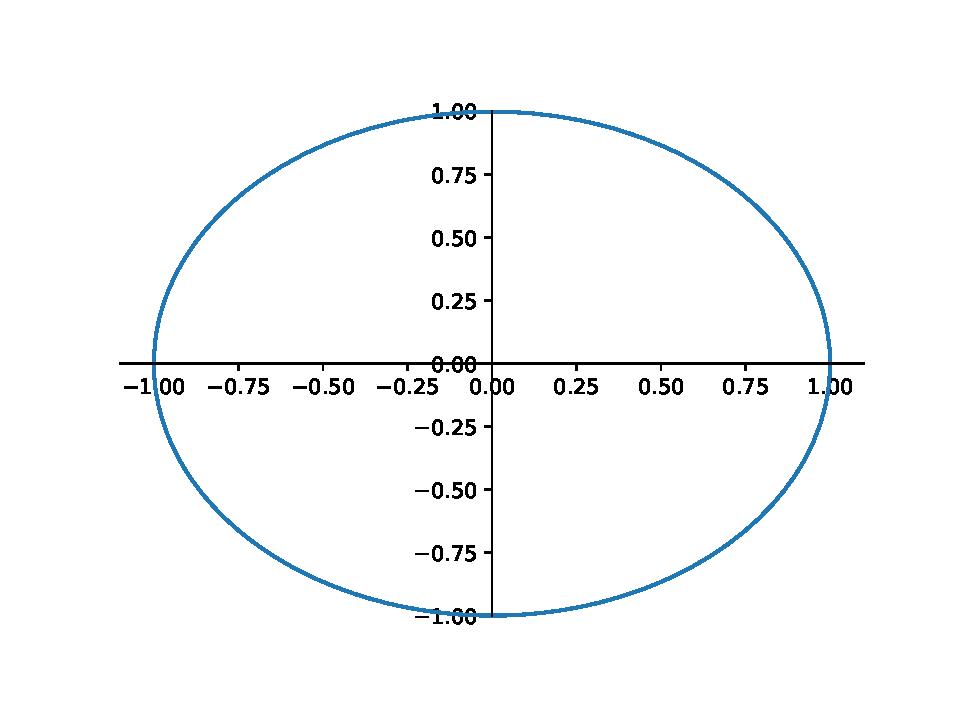
\includegraphics[width=\textwidth]{beamer-pics/conics-ellipse.pdf}
          \end{figure}
        \end{column}

        \begin{column}{0.5\textwidth}
          \begin{itemize}[<+->]
            \item Equation (centre $(Q,R)$): $\frac{(x-Q)^2}{a^2} + \frac{(y-R)^2}{b^2} = 1$
            \item Parametric form: $(Q + a\cos\theta,R + b\sin\theta)$
            \item Eccentricity: $e < 1$, $b^2 = a^2(1-e^2)$
            \item Focus: $(Q \pm ae,R)$
            \item Directrices: $x-Q = \pm\frac{a}{e}$
            \item Asymptotes: \textit{none}
          \end{itemize}
        \end{column}
      \end{columns}
    }
\end{frame}

\begin{frame}{Tangents and Normals}
  \begin{itemize}[<+->]
    \item The equation of the \textbf{tangent} to the curve $F(x)$ at the point $(A,B)$ is
    \begin{equation}
        y-B = \frac{dF}{dx}(x-A)
    \end{equation}
    where the gradient $\frac{df}{dx}$ is evaluated at the point $(A,B)$.
    \item The \textbf{tangent} and the \textbf{normal} are perpendicular, so the product of their gradients is $-1$.
    \item Thus, the equation of the \textbf{normal} to the curve $F(x)$ at the point $(A,B)$ is
    \begin{equation}
        y-B = k(x-a)
    \end{equation}
    where $k = -\frac{1}{\frac{dF}{dx}}$.
  \end{itemize}
\end{frame}

\end{document}
